% !TEX program = xelatex
% =====================================================================
%  PROJECT 3 – Truy vấn đa phương thức có giải thích bằng đồ thị
%  Slide trình bày theo template của nhóm (Beamer · Madrid · 16:9 · 10pt)
%  Compiler: XeLaTeX (chạy 2 lần)
% =====================================================================
\documentclass[10pt, aspectratio=169]{beamer}

% ── Font & ngôn ngữ ──────────────────────────────────────────────
\usepackage{fontspec}
\usepackage{polyglossia}
\setmainlanguage{vietnamese}
\setotherlanguage{english}
\setmainfont{Latin Modern Roman}
\setsansfont{Latin Modern Sans}
\setmonofont{Latin Modern Mono}

\usepackage{amsmath, amssymb}
\usepackage{bm}
\usepackage{xcolor}
\usepackage{booktabs}
\usepackage{multirow}
\usepackage{tikz}
\usetikzlibrary{positioning, arrows.meta, fit, calc}
\usepackage{pgfplots}
\pgfplotsset{compat=1.18}
\usepackage{adjustbox}

% ── Giao diện Slide (template) ───────────────────────────────────
\usetheme{Madrid}
\usecolortheme{default}
\setbeamertemplate{navigation symbols}{}

% ── Màu theo tông Madrid ─────────────────────────────────────────
\definecolor{xanh}{RGB}{51,51,178}
\colorlet{xanhnhat}{xanh!10}
\definecolor{cam}{RGB}{204,82,0}
\definecolor{xam}{RGB}{110,110,110}
\definecolor{do}{RGB}{178,34,34}

\newcommand{\nhanxet}[1]{\par\smallskip$\Rightarrow$ \textit{Nhận xét: #1}}
\newcommand{\code}[1]{\texttt{#1}}
\newcommand{\mrr}{MRR@100}
\newcommand{\pmm}{\ensuremath{\pm}}
\newcommand{\hinh}[2][0.66]{{\centering\adjustbox{max width=\linewidth, max totalheight=#1\textheight}{#2}\par}}

% ── Thông tin trang bìa ──────────────────────────────────────────
\title[Project 3 · Truy vấn đa phương thức + xAI]{Truy Vấn Đa Phương Thức\\Có Giải Thích Bằng Đồ Thị}
\subtitle{Đồ án môn Học máy với dữ liệu đồ thị -- Project 3}
\author[Nhóm Project 3]{
  \textbf{Học viên thực hiện:}\\
  \dots\\
  Nguyễn Phước Thiện (25C15060)\\
  Quan Phú Long (25C15050)\\
  Trần Hồ Thanh Vũ (25C15068)\\[1ex]
  \textbf{Giáo viên hướng dẫn:} \dots
}
\institute[KHTN TP.HCM]{Trường Đại Học Khoa Học Tự Nhiên - ĐHQG TP.HCM}
\date{Tháng 11/2026}

\begin{document}

% ══════════════════════════════════════════════════════════════
\begin{frame}
  \titlepage
\end{frame}

\begin{frame}{Nội dung trình bày}
  \begin{columns}[T]
    \column{.48\textwidth}
      \tableofcontents
    \column{.5\textwidth}
      \begin{block}{Ba câu hỏi của đề}
        \begin{enumerate}
          \item \textbf{Truy vấn:} kết quả nào phù hợp nhất với truy vấn?
          \item \textbf{Vai trò đồ thị:} tri thức quan hệ giúp ở đâu?
          \item \textbf{Giải thích:} vì sao mô hình trả về kết quả này?
        \end{enumerate}
      \end{block}
      \begin{exampleblock}{Phạm vi}
        Nhánh A (văn bản $\to$ ảnh) trên Visual Genome và Flickr30k, thêm chiều ảnh $\to$ văn bản; chuyển giao sang MMKG di sản Việt Nam tự xây.
      \end{exampleblock}
  \end{columns}
\end{frame}

% ══════════════════════════════════════════════════════════════
\section{Bài toán và tiến độ}

\begin{frame}{Bài toán và động lực}
  \begin{itemize}
    \item CLIP tìm ảnh bằng cách so cosine giữa vectơ câu và vectơ ảnh.
    \item Hai giới hạn mà đề chỉ ra:
      \begin{enumerate}
        \item Không dùng \textbf{quan hệ có cấu trúc} giữa đối tượng và khái niệm.
        \item Không cho biết \textbf{vì sao} một ảnh được trả về.
      \end{enumerate}
    \item Đề yêu cầu: dùng đồ thị để \textbf{xếp hạng lại}, rồi giải thích bằng cạnh, đường đi hoặc đồ thị con đã \textbf{thật sự} tham gia vào việc xếp hạng.
  \end{itemize}
  \begin{exampleblock}{Ví dụ của đề}
    Truy vấn \textit{``a child playing football''}, nhưng trong ảnh chỉ nhận ra \textit{ball} và \textit{field}. Đường đi \textit{child -- plays -- football} trong đồ thị tri thức nối truy vấn với đúng bức ảnh.
  \end{exampleblock}
  \nhanxet{mục tiêu không phải xây mô hình thị giác mới, mà là \textbf{đo rõ vai trò của đồ thị}.}
\end{frame}

\begin{frame}{Tiến độ theo các cấp độ của đề}
  \centering\small
  \begin{tabular}{l p{6.0cm} l}
    \toprule
    \textbf{Cấp độ} & \textbf{Yêu cầu} & \textbf{Tình trạng} \\
    \midrule
    1 (7.0) & CLIP, đồ thị, GNN, xếp hạng lại, 3 seed, ablation, 5+5 truy vấn & \textcolor{xanh}{\textbf{Hoàn thành}} \\
    NV1 mở rộng & nDCG, ảnh $\to$ văn bản, nhóm truy vấn & \textcolor{xanh}{\textbf{Hoàn thành}} \\
    2 (8.5) & Tập công khai thứ hai (Flickr30k) & \textcolor{xanh}{\textbf{Hoàn thành}} \\
    2 (8.5) & Phương pháp từ năm 2024 (G-Retriever) & \textcolor{xanh}{\textbf{Hoàn thành}}, kết quả âm \\
    2 (8.5) & Bộ $\ge$20 truy vấn trực tiếp/gián tiếp & \textcolor{cam}{Đang làm} trên VG; có 318 câu trên MMKG \\
    3 (10) & Fidelity, validity, sparsity trên $\ge$10 truy vấn & \textcolor{xanh}{\textbf{Hoàn thành}} (val + test) \\
    3 (10) & MMKG tiếng Việt tự xây & \textcolor{xanh}{\textbf{Hoàn thành}} \\
    4 (+1--2) & Cải tiến riêng & \textcolor{do}{Chưa làm} \\
    Sản phẩm & Giao diện demo (Gradio), slide & \textcolor{xanh}{\textbf{Hoàn thành}} \\
    \bottomrule
  \end{tabular}
\end{frame}

% ══════════════════════════════════════════════════════════════
\section{Dữ liệu và chống rò rỉ}

\begin{frame}{Visual Genome và split cố định}
  \begin{columns}[T]
    \column{.5\textwidth}
      \begin{block}{Dữ liệu}
        \begin{itemize}
          \item 108.077 ảnh, 5,4 triệu câu mô tả vùng.
          \item Lấy 5 câu mỗi ảnh: 540.383 câu.
          \item Mã hoá một lần bằng OpenCLIP ViT-B/32 (đóng băng), lưu \code{.npz}.
        \end{itemize}
      \end{block}
    \column{.48\textwidth}
      \begin{block}{Split theo ảnh}
        \begin{itemize}
          \item Test 5.000 · Val 5.000 · Train 98.077.
          \item File split được commit, chạy lại cho ra file giống hệt.
        \end{itemize}
      \end{block}
  \end{columns}
  \begin{alertblock}{Ảnh trùng là nguồn rò rỉ}
    247 cặp ảnh có cosine $\ge 0{,}99$ (ví dụ ảnh 285982 và 2375578, cosine 0,99992). Hai bản của cùng một ảnh mà rơi vào train và test là rò rỉ. Nhóm gom các ảnh này thành nhóm, và cả nhóm luôn nằm cùng một tập.
  \end{alertblock}
\end{frame}

\begin{frame}{Giao thức đánh giá và quy tắc chống rò rỉ}
  \begin{columns}[T]
    \column{.5\textwidth}
      \textbf{Giao thức}
      \begin{itemize}
        \item Truy vấn: 25.000 câu của ảnh test; kho: 5.000 ảnh test.
        \item \textbf{Đáp án đúng:} mọi ảnh có câu trùng truy vấn (26\% câu bị trùng, như ``a man'').
        \item R@1/5/10, \mrr, nDCG@10.
        \item CLIP và CLIP + Graph dùng \textbf{cùng 100 ứng viên}.
      \end{itemize}
    \column{.48\textwidth}
      \textbf{Quy tắc (đề §6)}
      \begin{itemize}
        \item Từ vựng khái niệm, cạnh thống kê: chỉ đếm trên \textbf{train}.
        \item Mọi lựa chọn (lr, epoch, $\alpha$, explainer): trên \textbf{val}.
        \item Test chạy \textbf{đúng một lần} mỗi seed; script từ chối lần thứ hai.
        \item Quy tắc được commit \textbf{trước} khi chạy test.
      \end{itemize}
  \end{columns}
  \nhanxet{Recall tuyệt đối là cận dưới (chỉ xét 5 câu mỗi ảnh), nhưng so sánh giữa các mô hình vẫn công bằng.}
\end{frame}

\begin{frame}{Hai bộ dữ liệu bổ sung: Flickr30k và MMKG tiếng Việt}
  \begin{columns}[T]
    \column{.48\textwidth}
      \begin{block}{Flickr30k (tập công khai thứ hai)}
        \begin{itemize}
          \item 31.014 ảnh, 5 chú thích mỗi ảnh; cùng CLIP như VG.
          \item Chia lại theo cùng quy trình: train 21.014 · val 5.000 · test 5.000; gom 2 cặp ảnh gần trùng.
          \item Không có annotation đối tượng: chép nguyên 3.880 khái niệm từ đồ thị VG, nối mỗi ảnh với 16 khái niệm gần nhất (496.224 cạnh).
        \end{itemize}
      \end{block}
    \column{.5\textwidth}
      \begin{block}{MMKG di tích -- di sản Việt Nam (tự xây)}
        \begin{itemize}
          \item Thu từ Wikidata (\code{P1435}, \code{P17 = Q881}) và Wikimedia Commons; lưu snapshot thô rồi mới lọc.
          \item Duyệt: AI duyệt sơ bộ, một thành viên duyệt lại từng dòng (962 dòng).
          \item \textbf{119 thực thể} (80 hiện vật + 39 khái niệm), \textbf{303 bộ ba}, 17 quan hệ, \textbf{380 ảnh} giấy phép tự do.
          \item \textbf{318 truy vấn} sinh tự động: trực tiếp / gián tiếp $\times$ Anh / Việt; chỉ dùng để đánh giá.
        \end{itemize}
      \end{block}
  \end{columns}
  \nhanxet{data card đầy đủ (nguồn, giấy phép, cách tạo bộ ba) trong \code{data\_cards/mmkg\_vi.md}.}
\end{frame}

% ══════════════════════════════════════════════════════════════
\section{Phương pháp}

\begin{frame}{Pipeline tổng thể}
  \hinh[0.62]{%
  \begin{tikzpicture}[
    node distance=0.5cm and 0.55cm,
    box/.style={draw=xanh,thick,rounded corners=2pt,fill=xanhnhat,align=center,font=\small,minimum height=1.1cm,text width=2.4cm},
    data/.style={draw=xam,dashed,rounded corners=2pt,fill=gray!5,align=center,font=\small,text width=2.4cm,minimum height=0.9cm},
    arr/.style={-{Stealth[length=2.2mm]},thick,xanh}]
  \node[data] (q) {Truy vấn\\ văn bản $q$};
  \node[box,right=of q] (clip) {CLIP $f_T$\\ (đóng băng)};
  \node[box,right=of clip] (faiss) {FAISS\\ top-100 ảnh};
  \node[box,right=of faiss] (gnn) {GraphSAGE\\ điểm đồ thị $g$};
  \node[box,below=0.9cm of gnn] (fuse) {Kết hợp điểm\\ {\footnotesize $\alpha\cos+(1{-}\alpha)g$}};
  \node[box,left=of fuse] (exp) {Giải thích\\ (cạnh ảnh--khái niệm)};
  \node[box,left=of exp] (fid) {Đo fidelity,\\ validity, sparsity};
  \node[data,above=0.9cm of faiss] (img) {Ảnh $\to f_I$\\ (tính trước)};
  \node[data,above=0.9cm of gnn] (graph) {Đồ thị ảnh --\\ khái niệm};
  \draw[arr] (q) -- (clip); \draw[arr] (clip) -- (faiss); \draw[arr] (faiss) -- (gnn);
  \draw[arr] (img) -- (faiss); \draw[arr] (graph) -- (gnn);
  \draw[arr] (gnn) -- (fuse); \draw[arr] (fuse) -- (exp); \draw[arr] (exp) -- (fid);
  \end{tikzpicture}}
  \vfill
  \begin{block}{Đúng theo quy trình của đề (§4.2)}
    truy vấn $\to$ CLIP $\to$ top-$k$ theo cosine $\to$ điểm đồ thị $\to$ xếp hạng lại $\to$ giải thích $\to$ đo fidelity.
  \end{block}
\end{frame}

\begin{frame}{Đồ thị ảnh -- khái niệm}
  \begin{columns}[c]
    \column{.42\textwidth}
      \hinh[0.6]{%
      \begin{tikzpicture}[
        img/.style={draw=xanh,fill=xanhnhat,thick,minimum width=1.3cm,minimum height=0.9cm,font=\small},
        con/.style={draw=cam,fill=cam!12,rounded corners=6pt,font=\scriptsize,inner sep=3pt},
        arr/.style={-{Stealth[length=1.8mm]},thick,xam}]
      \node[img] (i) at (0,0) {Ảnh $i$};
      \foreach \t/\a in {man.n.01/150, jean.n.01/110, shirt.n.01/70, street.n.01/30, car.n.01/-10, \dots/-50} {
        \node[con] (c\a) at (\a:2.4) {\t};
        \draw[arr] (c\a) -- (i);
      }
      \node[con] (x) at (-2.6,-1.6) {sidewalk.n.01};
      \draw[arr,dashed,cam] (x) to[bend left=20] node[midway,left,font=\scriptsize,cam]{đồng xuất hiện} (c150);
      \node[font=\scriptsize,xam] at (0,-2.4) {16 khái niệm có cosine CLIP cao nhất};
      \end{tikzpicture}}
    \column{.56\textwidth}
      \begin{itemize}
        \item \textbf{Đỉnh:} mọi ảnh + 3.880 synset WordNet (gặp trong $\ge 5$ ảnh train). Vectơ khái niệm = CLIP của ``a photo of a \{lemma\}''.
        \item \textbf{Cạnh \code{contains}:} mỗi ảnh nối với \textbf{16 khái niệm gần nhất theo CLIP}, như nhau cho train/val/test.
          \begin{itemize}
            \item Ảnh mới chưa có nhãn vẫn dùng được.
            \item Không đọc annotation của test.
          \end{itemize}
        \item \textbf{Cạnh \code{cooccurs\_with}} (biến thể): cặp khái niệm cùng xuất hiện $\ge 10$ ảnh \textbf{train}, PMI $>0$, tối đa 10 láng giềng.
      \end{itemize}
  \end{columns}
\end{frame}

\begin{frame}{Mô hình: GraphSAGE một lớp, khởi tạo bằng CLIP}
  \begin{block}{Công thức}
    \[
      h_i = W_{\text{self}}\,x_i + b + \frac{1}{|N(i)|}\sum_{c\in N(i)} W_{\text{nb}}\,x_c,
      \qquad g(q,i)=\cos(f_T(q),h_i),
      \qquad s = \alpha\cos(f_T(q),x_i) + (1-\alpha)\,g
    \]
  \end{block}
  \begin{columns}[T]
    \column{.5\textwidth}
      \begin{itemize}
        \item Không hàm kích hoạt; CLIP đóng băng, chỉ học $W_{\text{self}}, W_{\text{nb}}, b$.
        \item Khởi tạo $W_{\text{self}}=I$, $W_{\text{nb}}=0$: lúc đầu $g$ \textbf{đúng bằng CLIP}.
        \item Một lớp, một chiều: ảnh test không ảnh hưởng lẫn nhau.
      \end{itemize}
    \column{.48\textwidth}
      \begin{itemize}
        \item \textbf{Loss:} InfoNCE trên ảnh đúng + 15 ảnh sai lấy từ top-100 CLIP, $\tau = 0{,}05$.
        \item Adam, early stopping theo \mrr{} val; lr $\in\{10^{-3},10^{-4}\}$ chọn trên val.
        \item $\alpha$ chọn trên val, lưới $0, 0{,}1, \dots, 1$.
      \end{itemize}
  \end{columns}
\end{frame}


\begin{frame}{Các mô hình đối chứng}
  \centering\small
  \begin{tabular}{l c p{8.2cm}}
    \toprule
    \textbf{Mô hình} & \textbf{lr} & \textbf{Trả lời câu hỏi} \\
    \midrule
    CLIP thuần & -- & Baseline \\
    Không đồ thị & $10^{-3}$ & $W_{\text{nb}} = 0$ cố định. Mức tăng đến từ đồ thị, hay chỉ từ phép chiếu học trên VG? \\
    \textbf{CLIP + Graph} & $10^{-4}$ & \textbf{Mô hình chính} \\
    + Đồng xuất hiện & $10^{-4}$ & Quan hệ khái niệm -- khái niệm có giúp thêm không? \\
    Đồ thị xáo cạnh & $10^{-4}$ & Ablation: xáo cạnh, giữ nguyên bậc, huấn luyện y hệt mô hình chính \\
    G-Retriever (PCST) & -- & Phương pháp 2024: đồ thị con phụ thuộc truy vấn \\
    \bottomrule
  \end{tabular}
  \vfill
  \begin{block}{Điều kiện so sánh}
    Cùng split, cùng 100 ứng viên, cùng định nghĩa đáp án, 3 seed (0, 1, 2), báo cáo mean $\pm$ std.
  \end{block}
\end{frame}

% ══════════════════════════════════════════════════════════════
\section{Kết quả Nhiệm vụ 1}

\begin{frame}{Văn bản $\to$ ảnh trên test}
  \centering\small
  \begin{tabular}{l c c c c}
    \toprule
    \textbf{Mô hình} & \textbf{R@1} & \textbf{R@5} & \textbf{R@10} & \textbf{\mrr} \\
    \midrule
    CLIP thuần & 0.0584 & 0.1422 & 0.2018 & 0.1076 \\
    Không đồ thị & 0.0689 \pmm{} 0.0006 & 0.1741 \pmm{} 0.0056 & 0.2457 \pmm{} 0.0043 & 0.1266 \pmm{} 0.0006 \\
    \textbf{CLIP + Graph} & 0.0705 \pmm{} 0.0014 & 0.1765 \pmm{} 0.0037 & \textbf{0.2492 \pmm{} 0.0015} & \textbf{0.1284 \pmm{} 0.0006} \\
    + Đồng xuất hiện & \textbf{0.0709 \pmm{} 0.0009} & \textbf{0.1792 \pmm{} 0.0012} & 0.2469 \pmm{} 0.0006 & 0.1280 \pmm{} 0.0006 \\
    Đồ thị xáo cạnh & 0.0686 \pmm{} 0.0002 & 0.1759 \pmm{} 0.0004 & 0.2489 \pmm{} 0.0004 & 0.1272 \pmm{} 0.0003 \\
    \bottomrule
  \end{tabular}
  \par\smallskip{\scriptsize\color{xam} 5.000 ảnh, 25.000 truy vấn, 3 seed. CLIP có std = 0 vì tất định.}
  \vfill
  \begin{block}{Đọc bảng}
    \begin{itemize}
      \item Mọi mô hình có học đều vượt CLIP rõ rệt: \mrr{} $+0{,}02$ (tăng tương đối khoảng 19\%).
      \item Giữa bốn mô hình có học, phần lớn mức chênh \textbf{nhỏ hơn hoặc xấp xỉ std}.
    \end{itemize}
  \end{block}
\end{frame}

\begin{frame}{nDCG@10 và chiều ảnh $\to$ văn bản}
  \centering\small
  \begin{tabular}{l c c c c}
    \toprule
    & \textbf{Văn bản $\to$ ảnh} & \multicolumn{3}{c}{\textbf{Ảnh $\to$ văn bản}} \\
    \cmidrule(lr){2-2}\cmidrule(lr){3-5}
    \textbf{Mô hình} & \textbf{nDCG@10} & \textbf{R@1} & \textbf{R@10} & \textbf{\mrr} \\
    \midrule
    CLIP thuần & 0.1169 & 0.1280 & 0.3630 & 0.2068 \\
    Không đồ thị & 0.1387 \pmm{} 0.0006 & 0.1484 \pmm{} 0.0015 & 0.3895 \pmm{} 0.0013 & 0.2281 \pmm{} 0.0006 \\
    CLIP + Graph & \textbf{0.1391 \pmm{} 0.0007} & 0.1515 \pmm{} 0.0008 & \textbf{0.3961 \pmm{} 0.0024} & 0.2315 \pmm{} 0.0007 \\
    + Đồng xuất hiện & 0.1383 \pmm{} 0.0006 & \textbf{0.1522 \pmm{} 0.0008} & 0.3957 \pmm{} 0.0016 & \textbf{0.2316 \pmm{} 0.0008} \\
    Đồ thị xáo cạnh & 0.1390 \pmm{} 0.0003 & 0.1519 \pmm{} 0.0009 & 0.3957 \pmm{} 0.0012 & 0.2312 \pmm{} 0.0010 \\
    \bottomrule
  \end{tabular}
  \vfill
  \begin{itemize}
    \item Chiều ảnh $\to$ văn bản không huấn luyện thêm; $\alpha$ chọn riêng trên val (0,6).
    \item Ba mô hình có đồ thị cao hơn mô hình không đồ thị khoảng 0,003 \mrr, nhưng bản xáo cạnh cũng đạt mức đó.
  \end{itemize}
  \nhanxet{trên toàn tập, nhóm không kết luận mô hình có học nào vượt trội.}
\end{frame}

% ══════════════════════════════════════════════════════════════
\section{Kết quả Nhiệm vụ 2: vai trò của đồ thị}

\begin{frame}{Mức tăng thật sự đến từ đâu?}
  \begin{columns}[c]
    \column{.55\textwidth}
      \hinh[0.62]{%
      \begin{tikzpicture}
      \begin{axis}[ybar, width=8cm, height=5.6cm, bar width=15pt,
        ymin=0.10, ymax=0.132, ylabel={\mrr{} (test)},
        symbolic x coords={a,b,c,d,e}, xtick=data,
        xticklabels={CLIP,Không đồ thị,Xáo cạnh,Đồng xuất hiện,CLIP + Graph},
        x tick label style={font=\scriptsize,align=center,text width=1.4cm},
        y tick label style={/pgf/number format/fixed,/pgf/number format/precision=3,font=\scriptsize},
        nodes near coords, nodes near coords style={font=\tiny,/pgf/number format/fixed,/pgf/number format/fixed zerofill,/pgf/number format/precision=4},
        enlarge x limits=0.14, axis lines*=left, ymajorgrids, grid style={gray!25}]
      \addplot[fill=xanh!70,draw=xanh,error bars/.cd,y dir=both,y explicit]
       coordinates {(a,0.1076)+-(0,0) (b,0.1266)+-(0,0.0006) (c,0.1272)+-(0,0.0003) (d,0.1280)+-(0,0.0006) (e,0.1284)+-(0,0.0006)};
      \end{axis}
      \end{tikzpicture}}
    \column{.43\textwidth}
      \begin{block}{Phân rã mức tăng +0,0208}
        \begin{itemize}
          \item \textbf{Phép chiếu học được:} +0,0190 (khoảng 91\%).
          \item \textbf{Đồ thị:} +0,0018 (khoảng 9\%).
        \end{itemize}
      \end{block}
      \begin{alertblock}{Lưu ý}
        Nếu không có mô hình đối chứng không đồ thị, toàn bộ mức tăng 19\% sẽ bị gán nhầm cho đồ thị.
      \end{alertblock}
  \end{columns}
\end{frame}

\begin{frame}{Ablation: đồ thị thật và đồ thị xáo cạnh}
  \centering\small
  \begin{tabular}{c c c c c}
    \toprule
    \textbf{Seed} & \textbf{Thật} & \textbf{Xáo} & \textbf{Không đồ thị} & \textbf{Thật -- xáo} \\
    \midrule
    0 & 0.1279 & 0.12681 & 0.1259 & +0.00109 \\
    1 & 0.1283 & 0.12735 & 0.1269 & +0.00095 \\
    2 & 0.1291 & 0.12736 & 0.1271 & +0.00174 \\
    \midrule
    Trung bình & 0.1284 & 0.12718 & 0.1266 & \textbf{+0.00126 \pmm{} 0.00042} \\
    \bottomrule
  \end{tabular}
  \vfill
  \begin{columns}[T]
    \column{.5\textwidth}
      \begin{block}{Kết quả}
        Đồ thị thật hơn bản xáo ở \textbf{cả 3 seed}. Với đồ thị xáo, $\alpha$ chọn được cao hơn và epoch tốt nhất muộn hơn: mô hình dựa vào CLIP nhiều hơn.
      \end{block}
    \column{.48\textwidth}
      \begin{alertblock}{Giới hạn}
        Chỉ 3 seed và một bản xáo; hiệu ứng khoảng 1\% \mrr. Nhóm dùng chữ ``phù hợp với giả thuyết'', không dùng ``chứng minh''.
      \end{alertblock}
  \end{columns}
\end{frame}

\begin{frame}{Đồ thị giúp ở nhóm truy vấn nào?}
  \centering\small
  \begin{tabular}{l r c c c c}
    \toprule
    \textbf{Nhóm} & $n$ & \textbf{CLIP} & \textbf{Không đồ thị} & \textbf{Xáo cạnh} & \textbf{CLIP + Graph} \\
    \midrule
    \textbf{generic} (nhiều ảnh đúng) & 2.820 & 0.0681 & 0.0914 \pmm{} 0.0092 & 0.0951 \pmm{} 0.0018 & \textbf{0.1082 \pmm{} 0.0040} \\
    specific (1 ảnh đúng) & 22.180 & 0.1126 & 0.1311 \pmm{} 0.0007 & 0.1313 \pmm{} 0.0005 & 0.1309 \pmm{} 0.0011 \\
    \midrule
    action & 2.217 & 0.1223 & 0.1446 \pmm{} 0.0004 & 0.1468 \pmm{} 0.0003 & 0.1455 \pmm{} 0.0012 \\
    \textbf{spatial} & 9.934 & 0.1158 & 0.1396 \pmm{} 0.0020 & 0.1410 \pmm{} 0.0007 & \textbf{0.1444 \pmm{} 0.0008} \\
    none & 12.849 & 0.0987 & 0.1134 \pmm{} 0.0011 & 0.1131 \pmm{} 0.0006 & 0.1130 \pmm{} 0.0012 \\
    \bottomrule
  \end{tabular}
  \par\smallskip{\scriptsize\color{xam} \mrr{} văn bản $\to$ ảnh trên test. Luật chia nhóm được chốt trên val trước khi chạy test.}
  \vfill
  \begin{exampleblock}{Điểm sáng: câu chung chung như ``a man'', ``white clouds''}
    Đồ thị thật tách rõ khỏi hai đối chứng; R@1 tăng khoảng 50\% (0,042 so với 0,027--0,028). Vectơ trung bình của 16 khái niệm giúp đẩy lên các ảnh \textit{thực sự chứa} khái niệm được nhắc tới.
  \end{exampleblock}
\end{frame}

\begin{frame}{Độ nhạy theo trọng số $\alpha$}
  \begin{columns}[c]
    \column{.55\textwidth}
      \hinh[0.65]{%
      \begin{tikzpicture}
      \begin{axis}[width=8cm,height=5.6cm,xlabel={$\alpha$},ylabel={\mrr{} val (TB 3 seed)},
        xmin=-0.03,xmax=1.03,ymin=0.104,ymax=0.13,legend pos=south west,legend style={font=\scriptsize},
        y tick label style={/pgf/number format/fixed,/pgf/number format/precision=3,font=\scriptsize},
        x tick label style={font=\scriptsize},ymajorgrids,grid style={gray!25}]
      \addplot[thick,xanh,mark=*] coordinates {(0,0.12763) (0.1,0.12680) (0.2,0.12630) (0.5,0.12323) (1,0.1061)};
      \addlegendentry{Đồ thị thật}
      \addplot[thick,do,mark=square*,dashed] coordinates {(0,0.12383) (0.1,0.12403) (0.2,0.12387) (0.5,0.12237) (1,0.1061)};
      \addlegendentry{Đồ thị xáo}
      \end{axis}
      \end{tikzpicture}}
    \column{.43\textwidth}
      \begin{itemize}
        \item $\alpha$ chọn được: 0 / 0 / 0,1 (thật), 0,1 / 0,2 / 0,1 (xáo).
        \item $\alpha \approx 0$: điểm cuối gần như chỉ còn nhánh đồ thị.
        \item CLIP \textbf{không bị bỏ}: vectơ CLIP của ảnh vẫn nằm trong $h_i$ qua $W_{\text{self}}$.
        \item Đường cong gần như phẳng trong $[0; 0{,}2]$.
      \end{itemize}
  \end{columns}
\end{frame}

\begin{frame}{Tập thứ hai: Flickr30k (test, 3 seed)}
  \centering\small
  \begin{tabular}{l c c c c}
    \toprule
    \textbf{Mô hình} & \textbf{R@1} & \textbf{R@10} & \textbf{\mrr} & $\alpha$ \\
    \midrule
    CLIP thuần & 0.4901 & 0.8250 & 0.6045 & 1 \\
    \textbf{Không đồ thị} & \textbf{0.5332 \pmm{} 0.0006} & \textbf{0.8556 \pmm{} 0.0011} & \textbf{0.6447 \pmm{} 0.0003} & 0,6 \\
    CLIP + Graph & 0.5309 \pmm{} 0.0036 & 0.8553 \pmm{} 0.0026 & 0.6432 \pmm{} 0.0028 & 0,5 \\
    Đồ thị xáo cạnh & 0.5276 \pmm{} 0.0014 & 0.8526 \pmm{} 0.0009 & 0.6399 \pmm{} 0.0015 & 0,4--0,5 \\
    \bottomrule
  \end{tabular}
  \par\smallskip{\scriptsize\color{xam} Cấu hình chép nguyên từ VG, không chỉnh siêu tham số; epoch và $\alpha$ chọn trên val, test chạy một lần.}
  \vfill
  \begin{columns}[T]
    \column{.5\textwidth}
      \begin{block}{Lặp lại kết luận của VG}
        \mrr{} 0,6045 $\to$ 0,6447 (+6,6\%), gần như toàn bộ nhờ phép chiếu học được.
      \end{block}
    \column{.48\textwidth}
      \begin{alertblock}{Khác VG}
        Đồ thị không thêm gì: Graph -- không đồ thị $= -0{,}0015 \pmm{} 0{,}0028$. Đồ thị thật vẫn hơn bản xáo (+0,0033 \pmm{} 0,0013), nhưng bản xáo kém cả mô hình không đồ thị.
      \end{alertblock}
  \end{columns}
\end{frame}

\begin{frame}{Phương pháp năm 2024: G-Retriever (PCST)}
  \begin{columns}[T]
    \column{.5\textwidth}
      \begin{block}{Tái lập 3 bước đầu (bỏ bước sinh câu bằng LLM)}
        \begin{enumerate}\small
          \item Gán thưởng cho $k$ khái niệm liên quan nhất với truy vấn.
          \item PCST (\code{pcst\_fast}) chọn cây liên thông $S_q$ trên đồ thị đồng xuất hiện; giữ cả đỉnh ``cầu nối''.
          \item Chấm ứng viên theo $S_q$: GĐ1 tỉ lệ khái niệm thuộc $S_q$; GĐ2 GraphSAGE chỉ gộp khái niệm trong $S_q$.
        \end{enumerate}
      \end{block}
      {\scriptsize Chọn trong 9 ứng viên (NativE, AdaMF-MAT, \dots): G-Retriever 33/40 điểm.}
    \column{.48\textwidth}
      \begin{alertblock}{Kết quả âm (theo quy tắc dừng đã chốt)}
        \begin{itemize}\small
          \item \textbf{GĐ1:} cả 9 lượt val chọn $\alpha = 1$ (= CLIP). Chênh điểm CLIP giữa hai ứng viên liền kề có trung vị 0,00037; tỉ lệ chạm $S_q$ quá thô.
          \item \textbf{GĐ2, test VG:} \mrr{} 0,1278 \pmm{} 0,0005, ngang đối chứng không đồ thị 0,1277 \pmm{} 0,0001.
          \item \textbf{GĐ2, Flickr30k:} 0,6408 \pmm{} 0,0003, thấp hơn đối chứng 0,6430 \pmm{} 0,0016.
        \end{itemize}
      \end{alertblock}
  \end{columns}
  \nhanxet{đồ thị con phụ thuộc truy vấn không mang thêm thông tin so với phép chiếu học được.}
\end{frame}

% ══════════════════════════════════════════════════════════════
\section{Kết quả Nhiệm vụ 3: giải thích}

\begin{frame}{Giải thích phải đến từ chính cơ chế xếp hạng}
  \begin{alertblock}{Đề cấm}
    Sinh một đường đi hợp lý \textit{sau khi} đã có kết quả mà đường đi đó không ảnh hưởng tới dự đoán.
  \end{alertblock}
  \begin{enumerate}
    \item Giải thích là \textbf{tập cạnh khái niệm $\to$ ảnh} mà mô hình thật sự dùng. Explainer chạy lại đúng mô hình xếp hạng trên đồ thị đã sửa; không có heuristic tìm đường đi.
    \item \textbf{Chốt chặn khớp mô hình:} \mrr{} val tính lại phải bằng \textbf{từng bit} số đã lưu lúc huấn luyện. Sai checkpoint, sai đồ thị hay sai $\alpha$ đều bị dừng.
    \item \textbf{Kiểm tra bằng can thiệp:} bỏ cạnh giải thích thì điểm và hạng phải đổi đúng hướng.
  \end{enumerate}
  \nhanxet{explainer dùng: Occlusion (xoá từng cạnh), Integrated Gradients, GNNExplainer.}
\end{frame}

\begin{frame}{Cấp độ 1: 5 thành công và 5 thất bại (val)}
  \centering\small\setlength{\tabcolsep}{4pt}
  \begin{tabular}{l l c c c}
    \toprule
    & \textbf{Truy vấn} & \textbf{Hạng CLIP $\to$ Graph} & \textbf{Xoá 3 cạnh: hạng} & \textbf{Bỏ mọi cạnh: hạng} \\
    \midrule
    \multirow{5}{*}{\rotatebox{90}{Thành công}}
    & man in a grey shirt and blue jeans & 99 $\to$ 1 & 1 $\to$ 1 & 1 $\to$ 7 \\
    & Blue jacket with orange stripes & 100 $\to$ 3 & 3 $\to$ 5 & 3 $\to$ 5 \\
    & part of a trouser & 100 $\to$ 3 & 3 $\to$ 4 & 3 $\to$ 1 \\
    & a girl wearing blue jeans. & 99 $\to$ 3 & 3 $\to$ 3 & 3 $\to$ 3 \\
    & the grass beside the car & 98 $\to$ 3 & 3 $\to$ 3 & 3 $\to$ 8 \\
    \midrule
    \multirow{5}{*}{\rotatebox{90}{Thất bại}}
    & scattered waves in water & 7 $\to$ 100 & 100 $\to$ 100 & 100 $\to$ 96 \\
    & tall green and tan grass & 15 $\to$ 96 & 96 $\to$ 96 & 96 $\to$ 94 \\
    & wheel of car & 15 $\to$ 96 & 96 $\to$ 97 & 96 $\to$ 82 \\
    & a wooden sign & 12 $\to$ 92 & 92 $\to$ 95 & 92 $\to$ 34 \\
    & handicap parking sign on metal post & 15 $\to$ 95 & 95 $\to$ 98 & 95 $\to$ 75 \\
    \bottomrule
  \end{tabular}
  \par\smallskip{\scriptsize\color{xam} Hạng của ảnh đúng. Ở cả 15 ảnh được giải thích, xoá 3 cạnh Occlusion chọn đều làm điểm đồ thị giảm.}
\end{frame}

\begin{frame}{Đọc 5 + 5 truy vấn}
  \begin{columns}[T]
    \column{.5\textwidth}
      \begin{block}{Thành công}
        \begin{itemize}
          \item Chủ yếu nhờ \textbf{vectơ của chính ảnh} (phép chiếu), không nhờ cạnh.
          \item Bỏ mọi cạnh: ảnh vẫn ở hạng 7/5/1/3/8, so với 99/100/100/99/98 theo CLIP.
          \item Cạnh giúp 3/5 ca, không đổi 1 ca, kéo xuống 1 ca.
        \end{itemize}
      \end{block}
    \column{.48\textwidth}
      \begin{alertblock}{Thất bại}
        \begin{itemize}
          \item Chủ yếu do $\alpha = 0$ và phép chiếu; cạnh làm nặng thêm ở vài ca (``a wooden sign'': 34 $\to$ 92).
          \item Cạnh đúng nghĩa vẫn có thể kéo ảnh xuống (\code{grass.n.01}: $-0{,}0031$).
          \item Cạnh CLIP top-16 có nhiễu (\code{screen\_saver.n.01}).
        \end{itemize}
      \end{alertblock}
  \end{columns}
  \nhanxet{giải thích hiển thị đúng đồ thị mô hình dùng, kể cả phần nhiễu, nên chỉ giải thích được một phần các ca thất bại.}
\end{frame}

\begin{frame}{Cấp độ 3: đánh giá giải thích định lượng}
  \begin{columns}[T]
    \column{.4\textwidth}
      \textbf{Thước đo}
      \begin{itemize}\small
        \item \textbf{Fid$^+$}: bỏ giải thích thì điểm, hạng giảm bao nhiêu.
        \item \textbf{Fid$^-$}: chỉ giữ giải thích thì điểm đổi bao nhiêu.
        \item \textbf{Sparsity}, \textbf{validity}.
        \item \textbf{Đối chứng}: xoá cùng số cạnh ngẫu nhiên, Wilcoxon một phía.
      \end{itemize}
      {\scriptsize 20 truy vấn bốc ngẫu nhiên một lần, 3 seed; ảnh giải thích = ảnh hạng 1. Chọn explainer và $m$ trên val, test chạy một lần.}
    \column{.58\textwidth}
      \centering\scriptsize\setlength{\tabcolsep}{3pt}
      \begin{tabular}{l l c c c c}
        \toprule
        \textbf{Tập} & \textbf{Explainer} & \textbf{Fid$^+$} & \textbf{Hạng tụt} & \textbf{Fid$^-$} & $p$ \\
        \midrule
        val & Occlusion & 0,0192 (0,0004) & 3,47 (0,22) & $-0{,}0107$ & $3{\cdot}10^{-5}$ \\
        val & IG & 0,0192 (0,0004) & 3,47 (0,22) & $-0{,}0107$ & $3{\cdot}10^{-5}$ \\
        val & GNNExplainer & 0,0022 (0,0004) & 0,45 (0,22) & $-0{,}0008$ & 0,29 \\
        \textbf{test} & \textbf{IG} & \textbf{0,0225} (0,0006) & \textbf{2,57} (0,26) & $-0{,}0124$ & $5{\cdot}10^{-4}$ \\
        \bottomrule
      \end{tabular}
      \par{\tiny\color{xam} $m = 10$; trong ngoặc: xoá 10 cạnh ngẫu nhiên.}
      \begin{block}{Trên test (IG, $m=10$)}
        \begin{itemize}\small
          \item Fid$^+$ gấp $\sim$37 lần ngẫu nhiên; 20/20 truy vấn hơn ngẫu nhiên; 11/20 ảnh tụt hạng.
          \item Validity 100\%, sparsity 0,375 (10/16 cạnh).
          \item Fid$^-$ âm: 6 cạnh còn lại kéo ảnh xuống.
        \end{itemize}
      \end{block}
  \end{columns}
\end{frame}

% ══════════════════════════════════════════════════════════════
\section{Chuyển giao sang MMKG tiếng Việt}

\begin{frame}{Chuyển giao mô hình VG sang MMKG, không huấn luyện lại}
  \begin{columns}[T]
    \column{.38\textwidth}
      \begin{itemize}\small
        \item Trọng số và $\alpha$ giữ nguyên từ val VG; giao thức chốt trong ADR trước khi chạy.
        \item Đỉnh khái niệm: 119 thực thể MMKG; mỗi ảnh nối 16 thực thể gần nhất theo CLIP (không dùng nhãn).
        \item Hai lớp: dùng 303 bộ ba MMKG thay cạnh đồng xuất hiện.
      \end{itemize}
    \column{.6\textwidth}
      \centering\scriptsize\setlength{\tabcolsep}{3pt}
      \begin{tabular}{l c c c c}
        \toprule
        \textbf{\mrr} & \textbf{CLIP} & \textbf{Không ĐT} & \textbf{Một lớp} & \textbf{Hai lớp} \\
        \midrule
        Toàn bộ (318) & 0,2766 & 0,2861\pmm0,0035 & 0,2836\pmm0,0006 & \textbf{0,2872}\pmm0,0019 \\
        \midrule
        Trực tiếp, Anh (80) & \textbf{0,464} & 0,458 & 0,459 & 0,462 \\
        Gián tiếp, Anh (79) & 0,418 & 0,442 & 0,436 & \textbf{0,458} \\
        \quad chung chung (44) & 0,539 & 0,592 & 0,575 & \textbf{0,609} \\
        Trực tiếp, Việt (80) & \textbf{0,123} & 0,118 & 0,115 & 0,114 \\
        Gián tiếp, Việt (79) & 0,101 & \textbf{0,126} & 0,124 & 0,115 \\
        \bottomrule
      \end{tabular}
  \end{columns}
  \vfill
  \begin{columns}[T]
    \column{.5\textwidth}
      \begin{block}{Đọc bảng}
        Mọi mô hình học trên VG vượt CLIP (+2,5--3,8\%), nhưng đối chứng không đồ thị đã đạt 0,2861. Hai lớp (có bộ ba) chỉ nổi ở câu gián tiếp tiếng Anh.
      \end{block}
    \column{.48\textwidth}
      \begin{alertblock}{Câu tiếng Việt}
        CLIP \code{laion2b} đặt các câu tiếng Việt rất gần nhau (cosine TB 0,92 so với 0,70): \mrr{} rơi từ 0,464 xuống 0,123. Đồ thị không sửa được gốc rễ này.
      \end{alertblock}
  \end{columns}
\end{frame}

\begin{frame}{Giải thích trên MMKG (IG, $m = 10$, 3 seed)}
  \centering\small
  \begin{tabular}{l r c c c}
    \toprule
    \textbf{Nhóm} & \textbf{Số} & \textbf{Fid$^+$} & \textbf{Hạng tụt} & $p$ \\
    \midrule
    MMKG, toàn bộ & 954 & 0,0094 (0,0001) & 0,82 (0,10) & $\approx 10^{-59}$ \\
    \quad trực tiếp, Anh & 240 & 0,0090 (0,0003) & 0,68 (0,09) & $10^{-13}$ \\
    \quad gián tiếp, Anh & 237 & 0,0081 (0,0004) & 1,12 (0,12) & $7{\cdot}10^{-18}$ \\
    \quad trực tiếp, Việt & 240 & 0,0107 (0,0000) & 0,73 (0,08) & $3{\cdot}10^{-14}$ \\
    \quad gián tiếp, Việt & 237 & 0,0097 (0,0000) & 0,77 (0,11) & $4{\cdot}10^{-16}$ \\
    \midrule
    Visual Genome test & 60 & 0,0225 (0,0006) & 2,57 (0,26) & $5{\cdot}10^{-4}$ \\
    \bottomrule
  \end{tabular}
  \par\smallskip{\scriptsize\color{xam} Trong ngoặc: bỏ 10 cạnh ngẫu nhiên của cùng ảnh, lặp 20 lần. Mọi lựa chọn lấy nguyên từ val VG; chạy một lần.}
  \vfill
  \begin{columns}[T]
    \column{.5\textwidth}
      \begin{block}{Giải thích vẫn trung thực trên miền mới}
        Fid$^+$ gấp $\sim$90 lần ngẫu nhiên, đúng ở cả 4 nhóm; validity 100\%, sparsity 0,375.
      \end{block}
    \column{.48\textwidth}
      \begin{alertblock}{Trung thực $\neq$ đúng}
        Chỉ 18,6\% ảnh hạng 1 là ảnh đúng: giải thích cho biết vì sao \textit{mô hình} chọn ảnh, không phải vì sao ảnh đúng.
      \end{alertblock}
  \end{columns}
\end{frame}

% ══════════════════════════════════════════════════════════════
\section{Demo}

\begin{frame}{Demo: truy vấn $\to$ top-$k$ + đường đi giải thích}
  \begin{columns}[c]
    \column{.62\textwidth}
      \hinh[0.72]{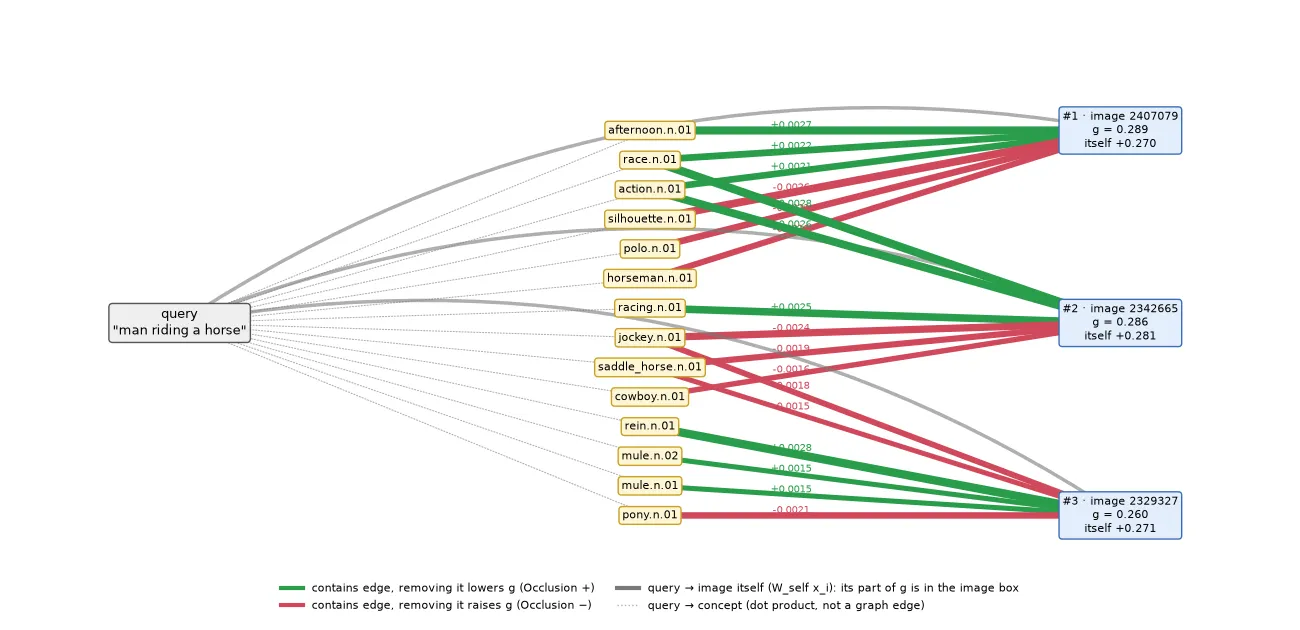
\includegraphics{../../results/figures/query_path.png}}
    \column{.36\textwidth}
      \begin{itemize}\small
        \item Gradio (\code{app/gradio\_app.py}), chạy được không cần GPU.
        \item Nhập câu, trả top-$k$ ảnh val và đường đi truy vấn $\to$ khái niệm $\to$ ảnh.
        \item \textcolor{xanh}{Cạnh xanh}: xoá thì $g$ giảm; \textcolor{do}{cạnh đỏ}: kéo ảnh xuống (Occlusion có dấu).
        \item Chỉ gọi hàm trong \code{src/mmxai/}: hiển thị đúng mô hình đã báo cáo.
      \end{itemize}
      {\scriptsize Ví dụ: ``man riding a horse''.}
  \end{columns}
\end{frame}

% ══════════════════════════════════════════════════════════════
\section{Hạn chế và hướng tiếp theo}

\begin{frame}{Hạn chế và hướng tiếp theo}
  \begin{columns}[T]
    \column{.55\textwidth}
      \begin{alertblock}{Hạn chế}
        \begin{enumerate}\small
          \item \textbf{Đồ thị đóng góp ít}: $\sim$91\% mức tăng trên VG đến từ phép chiếu; trên Flickr30k, MMKG và G-Retriever đồ thị không hơn mô hình không đồ thị.
          \item \textbf{Đồ thị ít ``quan hệ''}: cạnh suy từ chính CLIP, chưa có quan hệ scene graph, chưa dùng ConceptNet.
          \item \textbf{$\alpha$ cố định} gây các ca thất bại lớn (hạng 7--15 rơi xuống 92--100).
          \item \textbf{Thống kê}: 3 seed, một bản xáo, chưa kiểm định theo truy vấn.
          \item \textbf{Chưa xong}: bộ $\ge$20 truy vấn trên test VG; cấp độ 4.
        \end{enumerate}
      \end{alertblock}
    \column{.43\textwidth}
      \begin{exampleblock}{Hướng tiếp theo}
        \begin{itemize}\small
          \item \textbf{$\alpha(q)$ thích nghi theo truy vấn}.
          \item Thêm cạnh quan hệ scene graph + ConceptNet để kiểm giả thuyết ``đồ thị giàu quan hệ giúp truy vấn gián tiếp''.
          \item Bộ mã hoá văn bản đa ngôn ngữ cho truy vấn tiếng Việt (phải huấn luyện lại GNN).
        \end{itemize}
      \end{exampleblock}
  \end{columns}
\end{frame}

\begin{frame}{Kết luận}
  \begin{itemize}
    \item Visual Genome, quy trình chống rò rỉ chặt chẽ: \mrr{} test \textbf{0,1076 $\to$ 0,1284}.
    \item Đối chứng cho thấy $\sim$91\% mức tăng đến từ phép chiếu học được; cấu trúc ảnh -- khái niệm thật đóng góp \textbf{nhỏ nhưng nhất quán} so với đồ thị xáo, rõ nhất ở \textbf{truy vấn chung chung}.
    \item Kết luận ``phần lớn nhờ phép chiếu'' lặp lại trên \textbf{Flickr30k}, \textbf{MMKG tiếng Việt} và với \textbf{G-Retriever} (kết quả âm, báo cáo đúng quy tắc).
    \item Giải thích bằng \textbf{IG} tính trên chính mô hình xếp hạng: trên test VG và MMKG, bỏ cạnh giải thích làm tụt hạng \textbf{nhiều hơn rõ rệt} so với bỏ cạnh ngẫu nhiên.
  \end{itemize}
  \vfill
  \begin{block}{Mã nguồn}
    \url{https://github.com/FluteInTheRain/graph-semantic-image-editing}
  \end{block}
\end{frame}

\begin{frame}
  \centering\vspace{1cm}
  {\Huge\color{xanh} Cảm ơn thầy và các bạn đã lắng nghe!}\\[1cm]
  {\Large Hỏi đáp}
\end{frame}

\end{document}
